\subsection{Sensado}

La empresa requirió que se utilizara una ortesis de brazo donde se montara el sistema de medición de los sensores inerciales y la Raspberry Pi. La Figura \ref{fig:ortesis} muestra la ortesis de brazo utilizada. Para encontrar la posición del efector final, se utilizaron los dos sensores MPU-6050; uno se colocó en el codo, mientras que el segundo se colocó en el extremo de la ortesis. El sensor MPU-9250 se colocó en la parte superior de la mano, para controlar el movimiento del efector final.

\begin{figure}[htb]
	\centering
	\rotatebox{90}{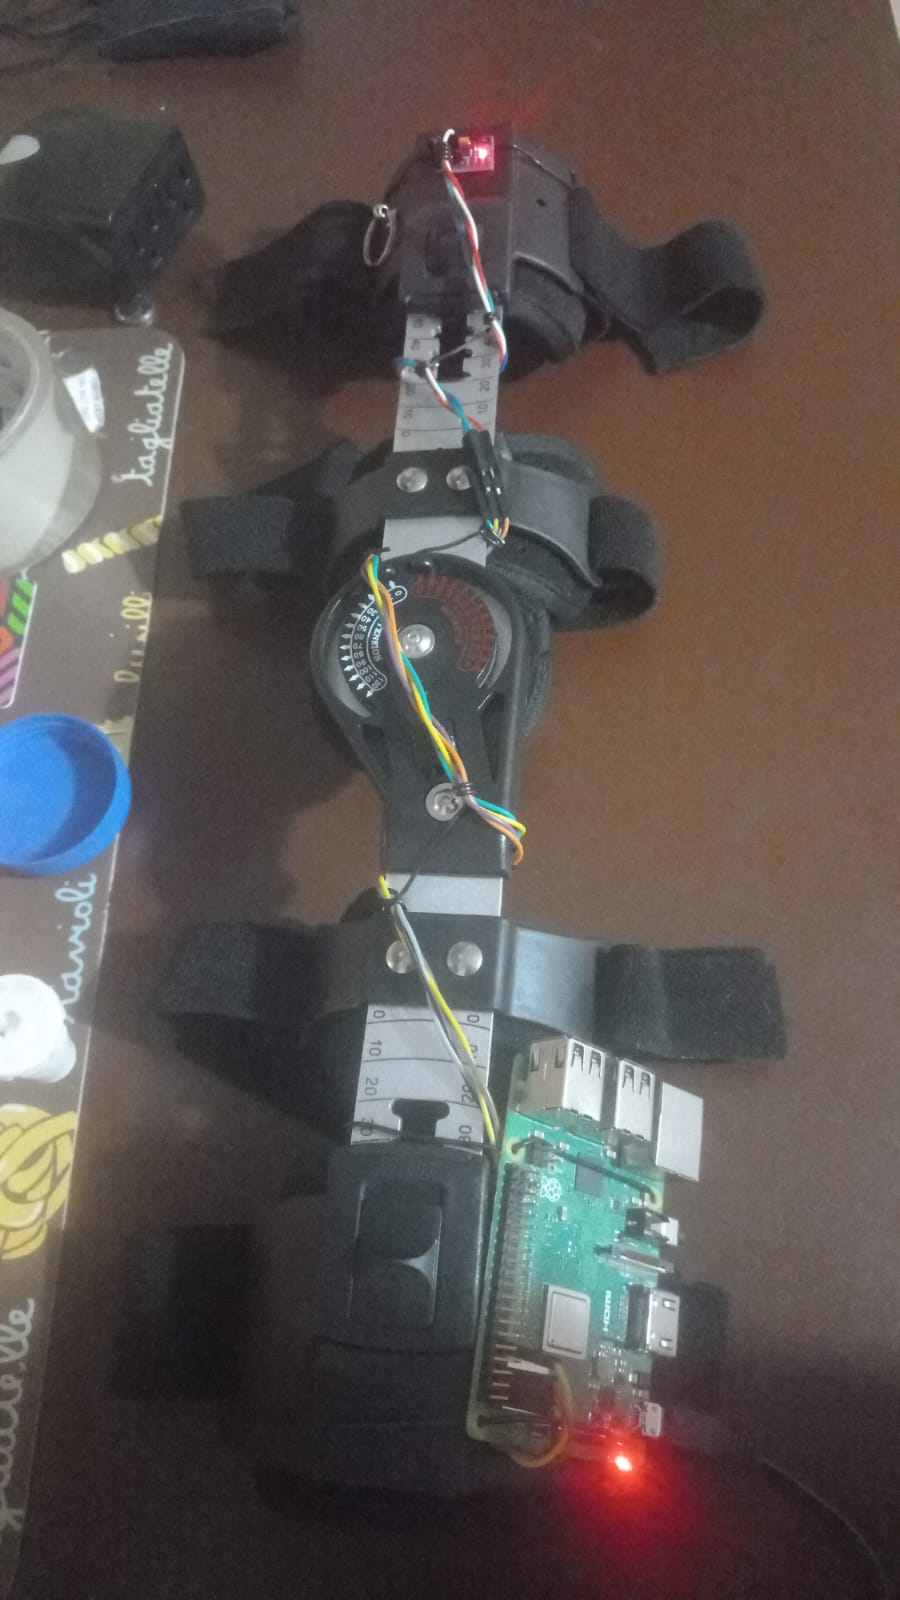
\includegraphics[scale=0.2]{ortesis.jpg}}
	\caption{Ortesis utilizada para el proyecto}
	\label{fig:ortesis}
\end{figure}

Se realizó la conexión entre los sensores y la Raspberry Pi 3 B+. La Figura \ref{fig:diagrama} muestra el diagrama de interconexión. Los pines SDA y SCL de los sensores MPU-6050 se conectaron al bus serial $I^2C$, mientras que los pines MISO, MOSI y SCK del sensor MPU-9250 se conectaron al bus serial SPI.

\begin{figure}[htb]
	\centering
	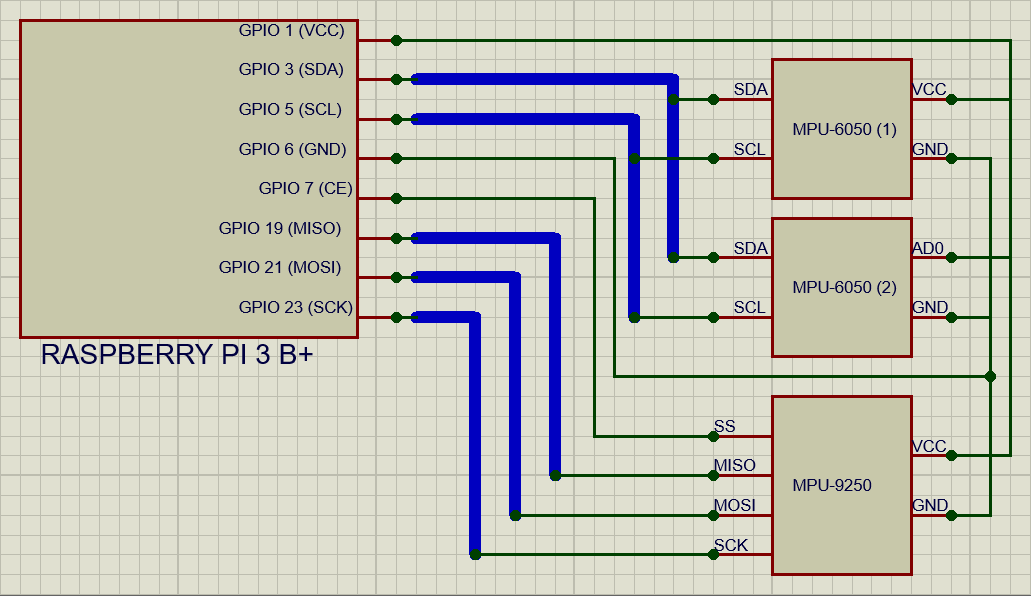
\includegraphics[scale=0.6]{diagrama.png}
	\caption{Diagrama de interconexión entre la Raspberry Pi y los sensores}
	\label{fig:diagrama}
\end{figure}

La línea SS del sensor MPU-9250 se conectó a la línea Chip Enable (CE) 1 de la Raspberry Pi. Nótese que tanto las líneas de datos (SDA), como las líneas de reloj (SCL) de los sensores MPU-6050, se conectaron a una única línea SDA o SCL, respectivamente, hacia la Raspberry Pi. Para evitar problemas de sincronización, se eligió la misma frecuencia de reloj para ambos sensores. Nótese también que se alimentó al sensor a través de la entrada AD0, en vez de VCC. Esto permite que su dirección en el bus $I^2C$ cambie de 104 a 105. Todos los sensores se alimentaron a través de la salida de voltaje de 3,3 V de la Raspberry Pi.

En lo que resta del documento, cuando se haga referencia a los sensores MPU-6050 y MPU-9250 en conjunto, se utilizará el prefijo MPU; cuando se haga referencia solo a uno de ellos, se hará con su nombre completo.

\subsubsection{Calibración}

Los sensores inerciales fabricados con tecnología MEMS, como los MPU, necesitan ser calibrados y tener un valor de referencia (offset) con el cual se corrija la orientación medida por el sensor \cite{offsetMPU}. El diagrama de la Figura \ref{fig:salidaMPU} obtenido del manual \cite{offsetMPU} muestra el proceso para obtener datos de los sensores MPU; los valores de referencia del acelerómetro y el giroscopio (Gyro and Accel Offset Registers) se aplican a las mediciones obtenidas por el giroscopio y el acelerómetro (Gyro and Accel MEMS), para corregir la mediciones y colocarlas en los registros del sensor (Gyro/Accel Output Registers). Luego, son procesadas por el Procesador de Movimiento Digital (DMP) y el resultado se almacena en un buffer FIFO interno.

\begin{figure}[htb]
	\centering
	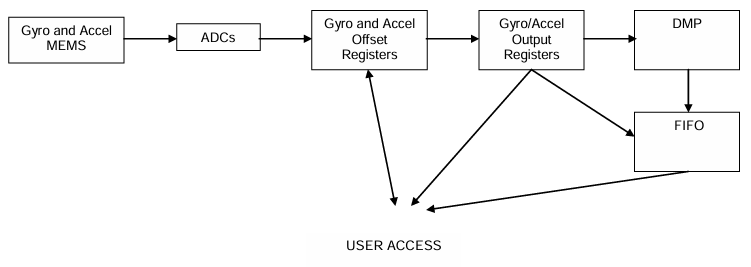
\includegraphics[scale=0.8]{salidaMPU.png}
	\caption{Lectura de datos de los sensores MPU}
	\label{fig:salidaMPU}
\end{figure}

%El buffer FIFO de los MPU permite implementar un patrón de arquitectura de segmentación de procesos (process pipeline); los datos obtenidos del DMP se colocan en un buffer interno del sensor de tipo FIFO (El primer dato que entra, es el último que sale), del cual se lee la orientación del sensor; esto permite que los datos de la orientación puedan ser procesados sin que existan errores debido a lecturas incompletas. Aunque no se indica explícitamente la estructura de datos interna del buffer, se puede representar como un buffer compartido, esto es, una cola circular. La Figura \ref{fig:buffer} muestra el buffer compartido. Puede notarse que se modela de tal manera que el proceso productor (el DMP) y el proceso consumidor (la lectura de datos del sensor) no accedan al mismo valor.

%\begin{figure}[htb]
%	\centering
%	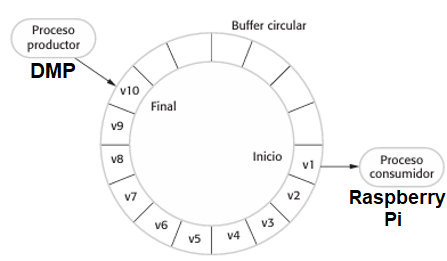
\includegraphics[scale=0.9]{buffer.png}
%	\caption{Representación del buffer interno del MPU como un buffer compartido}
%	\label{fig:buffer}
%\end{figure}

\newpage
La Figura \ref{fig:ejes} muestra los ejes de desplazamiento y la rotación de los sensores MPU. Se colocaron los sensores MPU en la ortesis de modo que el sentido positivo del eje X quedara hacia el frente del operador (quien tiene colocada la ortesis); de acuerdo con esto, el sentido positivo de rotación en el eje Z se obtiene girando el brazo hacia la izquierda del operador; el sentido positivo de rotación en el eje Y se obtiene girando el brazo hacia abajo; y el sentido positivo de rotación en el eje X se obtiene rotando el brazo hacia la derecha.

\begin{figure}[htb]
	\centering
	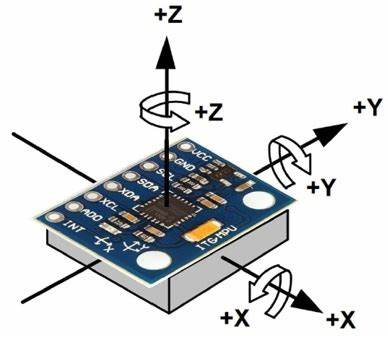
\includegraphics[scale=0.5]{ejes.jpeg}
	\caption{Orientación de los ejes y polaridad de rotación de los sensores MPU}
	\label{fig:ejes}
\end{figure}

Se eligieron los valores de referencia de modo que la salida del sensor en el inicio del proceso de medir la orientación fuera $X=0, Y=0, Z=0$ para el giroscopio y $X=0, Y=0, Z=-9.8$ para el acelerómetro, debido a la constante de la aceleración de la gravedad g = -9.8  $m/s^2$. De acuerdo con lo anterior, al procesar los datos por el DMP, la salida deseada en el inicio del proceso de medir la orientación sería $\theta_x = 0°,\theta_y = 0°,\theta_z = 0°$.

Si el sensor se encuentra en estado de reposo (no existe ninguna fuerza externa que lo mueva), se espera que al leer datos de él, los valores no cambien; en la práctica, estos valores pueden variar debido a interferencias como el ruido externo. De modo que se calcula un valor medio cuyo error (la diferencia entre la medición del sensor en estado de reposo y el valor medio) sea menor que un error máximo aceptable; con base en la experiencia, se eligió un error máximo de 0.1 $\degree/s$ para el giroscopio, y 0.1 $m/s$ para el acelerómetro.

Para obtener dicho valor medio, se utilizó un control proporcional-integral (PI), en el cual se escribe el valor medido por el sensor en los registros de referencia (offset registers), y se compara dicho valor con la siguiente medición del sensor (con el último offset escrito en los registros de referencia aplicado a la nueva medición), para determinar el error; este proceso termina cuando el error obtenido se encuentra dentro del rango previamente establecido.

La Figura \ref{fig:calibracion} muestra el proceso de calibración del sensor. A cada medición se le aplicó el control PI para corregir el error. Para permitir que se establezca un valor apropiado, este proceso se repite 600 veces, un valor elegido basado en la experiencia. Después de que termina el ciclo, se compara el siguiente valor del sensor con los valores de referencia en los registros para determinar el error. Si éste es mayor que el error máximo aceptado, se repite el proceso.

Para que la calibración sea adecuada y se obtenga una medición confiable, el sensor debe de encontrarse en el estado de reposo mencionado anteriormente.

\begin{figure}[htb]
	\centering
	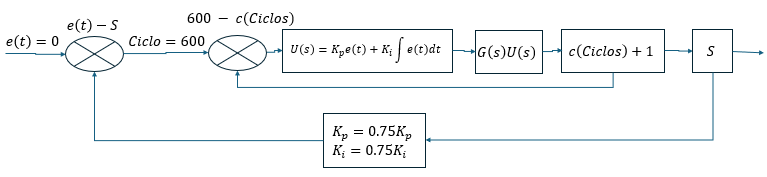
\includegraphics[scale=0.8]{calibracion.png}
	\caption{Diagrama a bloques del proceso de calibración del sensor}
	\label{fig:calibracion}
\end{figure}

<<<<<<< HEAD
=======
Se utilizó un patrón de arquitectura de segmentación de procesos (process pipeline), en el cual los datos obtenidos del DMP se colocan en un buffer interno del sensor de tipo FIFO (El primer dato que entra, es el último que sale), del cual se lee la orientación del sensor; esto permite que los datos de la orientación puedan ser procesados sin que existan errores debido a lecturas incompletas. Aunque no se indica explícitamente la estructura de datos interna del buffer, se puede representar como un buffer compartido, esto es, una cola circular. La Figura \ref{fig:buffer} muestra el buffer compartido. Puede notarse que se modela de tal manera que el proceso productor (el DMP) y el proceso consumidor (la lectura de datos del sensor) no accedan al mismo valor.

\begin{figure}[htb]
	\centering
	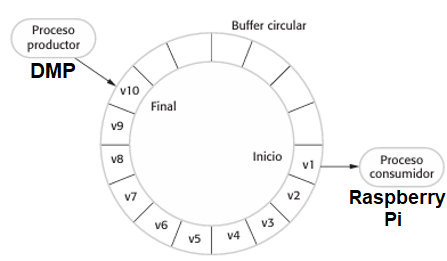
\includegraphics[scale=0.9]{buffer.png}
	\caption{Representación del buffer interno del MPU como un buffer compartido}
	\label{fig:buffer}
\end{figure}

\newpage
>>>>>>> texstudio
Posteriormente, se debe de cargar el firmware del procesador \cite{userguideMotionDriver}. Este proceso debe de realizarse cada vez que se encienda el sensor. Aunque no se indique explícitamente, el hecho de que el firmware deba de ser cargado cada vez que se inicie el sensor sugiere que la memoria que contiene el firmware del sensor es una memoria volátil. La memoria está formada por 8 bancos, en los que se carga el firmware proporcionado por InvenSense \cite{userguideMotionDriver}. 

Después de esto, se habilita el DMP y el buffer FIFO escribiendo el valor 1 en el bit FIFO\_EN (Bit 6) del registro 106 indicado en la Figura \ref{fig:fifoen} para la lectura de datos.

\begin{figure}[htb]
	\centering
	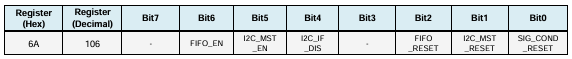
\includegraphics[scale=1]{fifoenable.png}
	\caption{Registro User Control del MPU, donde se encuentra el bit (Bit6) para activar el buffer FIFO}
	\label{fig:fifoen}
\end{figure}

\subsubsection{Medición}

El algoritmo utilizado por el DMP para obtener la orientación, no es de dominio público; en el Capítulo \ref{cap:anexos}, se describe el posible algoritmo utilizado por el DMP. Por otro lado, InvenSense, el desarrollador del sensor, ofrece un conjunto de bibliotecas para trabajar con el DMP \cite{userguideMotionDriver}.

%La Figura muestra el proceso general para obtener la orientación del sensor. Primero, se obtiene en el buffer FIFO la orientación obtenida por el DMP, representada internamente por un cuaternión. El cuaternión es rápidamente computable y evita problemas que se producen al girar más de 90°, como el bloqueo del cardán. Posteriormente, se obtiene el vector de gravedad; este permite calcular la aceleración de la gravedad que experimenta el sensor en los 3 ejes, para tomarlo como sesgo y corregir la medición. Por último, se convierte lo antes calculado a valores de Euler, en radianes, y finalmente, dichos valores son convertidos a su equivalente en grados, que son los que se utilizan para indicar la orientación del sensor.

%\begin{figure}[htb]
%	\centering
%	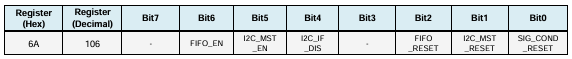
\includegraphics[scale=1]{fifoenable.png}
%	\caption{Determinación de la orientación del sensor}
%	\label{fig:orientacion}
%\end{figure}

El DMP representa internamente la orientación por medio de cuaterniones unitarios. Son rápidamente computables, y evitan problemas que se producen al girar más de 90\degree, como el bloqueo del cardán.

El cuaternión es de la forma:.

\begin{equation}
	q = a + b\hat{i} + c\hat{j} + d\hat{k}
	\label{eq:eqcuaternion}
\end{equation}

Donde $a, b, c, d$ son las componentes del cuaternión que describe la rotación actual del sensor.

Para poder obtener la rotación del sensor, se utilizó la formula que obtiene las nuevas componentes de un vector si se le aplica una rotación descrita por un cuaternión, la cual es la siguiente:

\begin{equation}
	v' = q\cdot v\cdot q*
	\label{eq:rotacioncuaternion}
\end{equation}

Donde $v'$ es el nuevo vector con la rotación aplicada, y $q*$ es el cuaternión conjugado, de la forma:

\begin{equation}
	q* = a - b\hat{i} - c\hat{j} - d\hat{k}
	\label{eq:eqcuaternionconj}
\end{equation}

De acuerdo con los valores de referencia definidos para el acelerómetro ($X=0, Y=0, Z=-9.8$), el vector de gravedad es $g = (0, 0, -1)$. Se sustituyó en la ecuación \ref{eq:rotacioncuaternion} $v$ por el vector de gravedad. Al resolver, se obtuvieron las siguientes ecuaciones para obtener cada componente del vector de gravedad:

\begin{equation}
	v'_x = 2\cdot(x \cdot z - w \cdot y)
	\label{eq:componentex}
\end{equation}

\begin{equation}
	v'_y = 2\cdot(w \cdot x + y \cdot z)
	\label{eq:componentey}
\end{equation}

\begin{equation}
	v'_z = w^2 - x^2 - y^2 + z^2
	\label{eq:componentez}
\end{equation}

Para obtener los ángulos entre el vector $v'$ y los ejes $x$, $y$, $z$ definidos cuando se calibró el sensor (es decir, aquella orientación del sensor en la que la salida del DMP es $\theta_x = 0°,\theta_y = 0°,\theta_z = 0°$), se utilizaron las siguientes ecuaciones:

\begin{equation}
	\theta_x = \tan^{-1}\frac{v'_y}{v'_z}
	\label{eq:angulox}
\end{equation}

\begin{equation}
	\theta_y = \tan^{-1}\frac{v'_x}{\sqrt{v'^2_y + v'^2_z}}
	\label{eq:anguloy}
\end{equation}

\begin{equation}
	\theta_z = \tan^{-1}\frac{q_x \cdot q_y + q_w \cdot q_z}{1 - 2 \cdot (q_x^2 + q_y^2)}
	\label{eq:anguloz}
\end{equation}

Si el sensor se encuentra boca abajo (es decir, la componente Z del vector de gravedad apunta en el sentido positivo del eje Z), es necesario invertir el sentido de la inclinación en el eje Y. Si el valor de la inclinación en el eje Y es positivo, el valor se corrige a $\pi - v'_y$; si es negativo, el valor se ajusta a $-\pi - v'_y$.

Los ángulos obtenidos $\theta_x$, $\theta_y$, $\theta_z$, son la orientación del sensor.